\documentclass[aspectratio=169, 11pt, xcolor=table]{ctexbeamer}

% Packages
\usepackage{graphicx}
\usepackage{booktabs}
\usepackage{xcolor}
\usepackage{tikz}
\usepackage{multicol}
\usepackage{listings}

% Fix for Fandol font italic issue
\xeCJKsetup{AutoFakeSlant}

% Theme settings - Metropolis minimalist style
\usetheme[progressbar=frametitle, block=fill, sectionpage=progressbar]{metropolis}
\setbeamertemplate{navigation symbols}{}
\setbeamertemplate{footline}[frame number]
\setbeamertemplate{bibliography item}{\insertbiblabel}

% Loosen vbox/hbox tolerance — metropolis 标题页内部 vbox 计算会产生 ~22pt 容差，纯日志噪音不影响显示
\vfuzz=50pt
\hfuzz=20pt

% TikZ libraries for diagram
\usetikzlibrary{shapes.geometric, arrows.meta, positioning, fit, backgrounds, calc}

% Define Global Academic Palette
\definecolor{JNUBlue}{RGB}{0, 85, 162} % 暨南大学标准蓝 (近似)
\definecolor{colorVector}{HTML}{FF6B6B}
\definecolor{colorGraph}{HTML}{4A90E2}
\definecolor{colorDRR}{HTML}{50E3C2}
\definecolor{colorHighlight}{HTML}{F39C12}

% Global styling
\setbeamerfont{block title}{shape=\normalfont, series=\bfseries}
\setbeamerfont{title}{shape=\normalfont, series=\bfseries, size=\Large}
\setbeamerfont{subtitle}{size=\small}
\setbeamerfont{author}{size=\small}
\setbeamerfont{institute}{size=\normalsize}
\setbeamerfont{date}{size=\footnotesize}

% Metropolis Theme Custom Colors
\setbeamercolor{normal text}{fg=darkgray!90!black}
\setbeamercolor{palette primary}{bg=JNUBlue, fg=white}
\setbeamercolor{progress bar}{fg=colorHighlight, bg=JNUBlue!30}
\setbeamercolor{title separator}{fg=colorHighlight, bg=JNUBlue}
\setbeamercolor{alerted text}{fg=colorVector}
\setbeamercolor{block title}{bg=JNUBlue!15, fg=JNUBlue!90!black}
\setbeamercolor{block body}{bg=JNUBlue!5, fg=darkgray!90!black}

% Graphic path
\graphicspath{{./figures/}}

% Title Page Info
\title{基于树--图双重表征推理的全栈智能知识平台}
\subtitle{\small 本科毕业论文答辩}

\author{%
    \small
    \textbf{答辩人：}沈宇飞\\
    \textbf{指导老师：}XXX 教授\\
    \textbf{专\qquad 业：}计算机科学与技术%
}
\institute{\large \textbf{暨南大学}}
\date{\footnotesize 2026年5月}

% 添加封面右上角的“树-图双重表征”科技感抽象 Logo
\titlegraphic{
    \begin{tikzpicture}[overlay, remember picture]
        \node[anchor=north east, xshift=-1cm, yshift=-1cm] at (current page.north east) {
            \begin{tikzpicture}[scale=0.6, every node/.style={circle, draw=JNUBlue, fill=JNUBlue!10, inner sep=2pt, minimum size=6pt}]
                % Tree nodes
                \node (root) at (0,0) {};
                \node (l1) at (-1.2,-1) {};
                \node (r1) at (1.2,-1) {};
                \node (l2) at (-1.8,-2) {};
                \node (m2) at (-0.6,-2) {};
                \node (r2) at (0.6,-2) {};
                \node (rr2) at (1.8,-2) {};
                
                % Tree edges (solid, downward)
                \draw[JNUBlue, thick] (root)--(l1) (root)--(r1);
                \draw[JNUBlue, thick] (l1)--(l2) (l1)--(m2);
                \draw[JNUBlue, thick] (r1)--(r2) (r1)--(rr2);
                
                % Graph edges (dashed, cross-domain connections representing DRR)
                \draw[colorVector, thick, dashed] (l2) to[bend right=20] (m2);
                \draw[colorVector, thick, dashed] (m2) to[bend left=15] (r2);
                \draw[colorVector, thick, dashed] (r2) to[bend right=20] (rr2);
                \draw[colorVector, thick, dashed] (l1) to[bend left=10] (r2);
            \end{tikzpicture}
        };
    \end{tikzpicture}
}




\begin{document}

\maketitle

\begin{frame}{汇报大纲}
    \tableofcontents
\end{frame}

% --- SECTION 1: 研究背景与痛点 ---
\section{研究背景与痛点}

\begin{frame}{跨域创新中的“语义鸿沟”}
    \small
    \begin{columns}[onlytextwidth]
        \column{0.48\textwidth}
        \textbf{核心痛点：} 
        当工程师提出“被动散热”或“可逆强黏附”等需求时，可借鉴机制往往分散在不同学科中，且很少以相同术语表达。
        
        \textbf{纯向量 RAG 的局限：}
        \begin{itemize}[<+->]
            \setlength{\itemsep}{0pt}
            \item \alert{语义漂移}：容易停留在表层名词匹配，难以命中深层机制。
            \item \alert{上下文割裂}：无法有效组织跨越多个文档的复杂机制链路。
            \item \alert{工程约束弱化}：生成的方案往往缺乏物理可行性与具体工程参数。
        \end{itemize}

        \column{0.48\textwidth}
        \vspace{-0.2cm}
        \begin{block}{案例引出：光刻机主动隔振系统}
            \small
            \textbf{核心难点}：负刚度机构与 Nyquist 控制稳定性的多物理场协同。\\
            \textbf{纯参数化输出}：通用的气浮隔振+线性二次型控制模板（忽略硬约束）。\\
            \textbf{DRR 工程交付}：被动负刚度 + 主动反馈混合架构，精确覆盖共振与相位裕度约束。
        \end{block}
    \end{columns}
\end{frame}

% --- SECTION 2: 核心方法 ---
\section{核心方法：MTGCR 与 DRR 链路}

\begin{frame}{机制树引导的社区检索与约束收束 (MTGCR)}
    \textbf{核心思想}：先用树结构收缩问题空间，再用社区级图检索扩展机制邻域，最后通过严格的约束审查完成工程收束。
    
    \vspace{0.3cm}
    \begin{block}{候选压缩与约束满足的统一框架}
        \small
        \begin{enumerate}[<+->]
            \item \textbf{机制树生成 ($T$)}：$T = \mathrm{LLM}_{\mathrm{tree}}(q; P_{\mathrm{tree}})$
            \item \textbf{活性成分抽取 ($A$)}：提取机制锚点 $A = g(T)$
            \item \textbf{社区级图检索 ($R$)}：$R = h(q, A, \mathcal{G}_{base}, \mathcal{C})$，基于 GraphRAG 扩展邻域。
            \item \textbf{草稿生成 ($\hat{y}$)}：$\hat{y} = \mathrm{LLM}_{\mathrm{draft}}(q, R; P_{\mathrm{draft}})$
            \item \textbf{约束批评与工程交付 ($y$)}：$y = \mathrm{LLM}_{\mathrm{refine}}(q, R, \hat{y}; P_{\mathrm{refine}})$
        \end{enumerate}
    \end{block}
\end{frame}

% --- SECTION 3: 系统架构 ---
\section{全栈平台架构与实现}

\begin{frame}[fragile]{全栈智能知识平台总体架构}
    \centering
    \resizebox{0.95\textwidth}{!}{%
    \begin{tikzpicture}[
        node distance=0.45cm and 0.7cm,
        block/.style={rectangle, draw, rounded corners=3pt, minimum height=0.75cm, minimum width=1.85cm, font=\small, fill=#1!15, draw=#1!60, line width=0.5pt, text width=1.9cm, align=center},
        block/.default=blue,
        decision/.style={diamond, draw, aspect=2.1, inner sep=1.2pt, font=\small, fill=orange!15, draw=orange!60, line width=0.5pt},
        arrow/.style={-{Stealth[length=4pt]}, semithick, color=gray!75},
        annot/.style={font=\scriptsize\itshape, text=gray!80}
    ]
    \node[block=violet] (query) {工程问题输入};
    \node[decision, right=of query] (router) {任务路由};

    \node[block=teal, above right=0.4cm and 1.0cm of router] (tree) {Mechanism Trees\\局部机制分解};
    \node[block=blue, below right=0.4cm and 1.0cm of router] (hybrid) {Hybrid Retrieval\\混合检索};

    \node[block=teal, right=of tree] (ingredient) {活性成分\\提取与整理};
    \node[block=blue, right=0.75cm of ingredient, yshift=-0.82cm] (graphrag) {GraphRAG\\社区级全局检索};

    \node[block=green, right=of graphrag] (draft) {DRR\_Draft\\草稿生成};
    \node[block=red, right=of draft] (critic) {主路线选择\\约束批评};
    \node[block=green, right=of critic] (delivery) {工程交付\\细节补足};

    \draw[arrow] (query) -- (router);
    \draw[arrow] (router) |- node[above, annot, xshift=0.3cm, yshift=0.05cm] {复杂工程} (tree);
    \draw[arrow] (router) |- node[below, annot, xshift=0.3cm, yshift=-0.05cm] {通用问答} (hybrid);

    \draw[arrow] (tree) -- (ingredient);
    \draw[arrow] (ingredient) -| (graphrag);
    \draw[arrow] (hybrid) -- (graphrag);
    \draw[arrow] (graphrag) -- (draft);
    \draw[arrow] (draft) -- (critic);
    \draw[arrow] (critic) -- (delivery);

    \node[block=gray, below=0.6cm of graphrag, text width=3.5cm] (db) {Neo4j / PostgreSQL\\语料与图谱持久化};
    \draw[arrow, dashed, <->] (graphrag) -- (db);
    \draw[arrow, dashed, <->] (hybrid) |- (db);
    
    % Boundary boxes
    \begin{scope}[on background layer]
        \node[draw=teal!50, fill=teal!5, rounded corners, fit=(tree) (ingredient), inner sep=0.25cm] (box1) {};
        \node[above left, annot, color=teal!80!black] at (box1.north east) {局部机制表示};
        
        \node[draw=blue!50, fill=blue!5, rounded corners, fit=(hybrid) (graphrag), inner sep=0.25cm] (box2) {};
        \node[above left, annot, color=blue!80!black] at (box2.north east) {全局图谱检索};
        
        \node[draw=red!50, fill=red!5, rounded corners, fit=(draft) (critic) (delivery), inner sep=0.25cm] (box3) {};
        \node[above left, annot, color=red!80!black] at (box3.north east) {非对称生成与约束收束};
    \end{scope}
    \end{tikzpicture}
    }
    
    \vspace{0.3cm}
    \small \textbf{图表说明}：本图展示了全栈平台的完整推理与生成流程。左侧为基于树的机制分解，中侧为基于图谱的全局检索，右侧为非对称的“草稿-批评-交付”生成链路。
\end{frame}

% --- SECTION 4: 实验分析 ---
\section{实验设计与结果分析}

\begin{frame}{自动评分结果：一致的相对提升}
    \small
    \begin{columns}[T,onlytextwidth]
        \column{0.48\textwidth}
        \centering
        \setlength{\fboxsep}{0pt}
        \setlength{\fboxrule}{0.5pt}
        \fcolorbox{gray!30}{white}{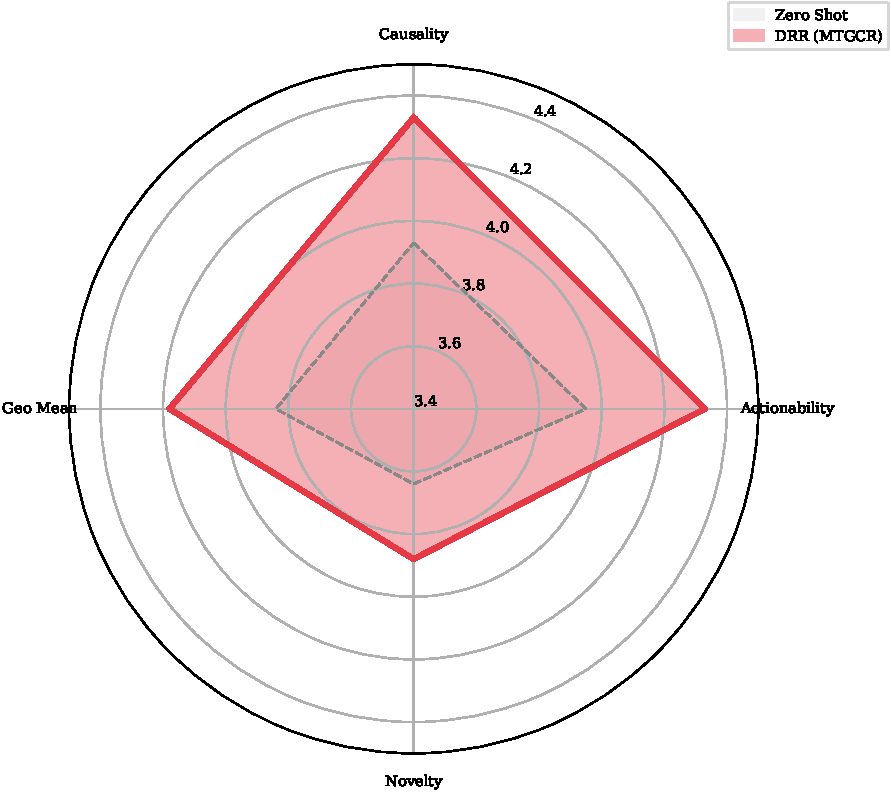
\includegraphics[width=0.95\textwidth]{thesis_main_radar_zoomed.pdf}}
        
        \vspace{0.2cm}
        \begin{beamercolorbox}[wd=\textwidth, rounded=true, shadow=false, sep=0.5ex]{block body}
            \scriptsize \textbf{图表说明}：DRR 与基线在三大核心维度上的能力雷达对比，展现了系统级的全面包络优势。
        \end{beamercolorbox}
        
        \column{0.48\textwidth}
        \textbf{核心指标提升 (42题)}：
        \begin{itemize}[<+->]
            \setlength{\itemsep}{0pt}
            \item \textbf{因果清晰度}：3.93 $\rightarrow$ 4.33 (\alert{+10.2\%})
            \item \textbf{工程可执行性}：3.95 $\rightarrow$ 4.33 (\alert{+9.6\%})
            \item \textbf{创新性}：3.64 $\rightarrow$ 3.88 (\alert{+6.6\%})
        \end{itemize}
        
        \vspace{0.2cm}
        \textbf{分层表现差异}：
        \begin{itemize}[<+->]
            \setlength{\itemsep}{0pt}
            \item 在 \textbf{开放探索题型} 提升最为显著。
            \item 在 \textbf{锚点工程题型} 中，DRR 在创新性上与基线打平（3.17 vs 3.33），表明系统在成熟题型中倾向于\alert{保留行业标准路线，不盲目追求新颖}。
        \end{itemize}
    \end{columns}
\end{frame}

\begin{frame}{模型表现分布：长尾鲁棒性}
    \small
    \begin{columns}[T,onlytextwidth]
        \column{0.54\textwidth}
        \centering
        \setlength{\fboxsep}{0pt}
        \setlength{\fboxrule}{0.5pt}
        \fcolorbox{gray!30}{white}{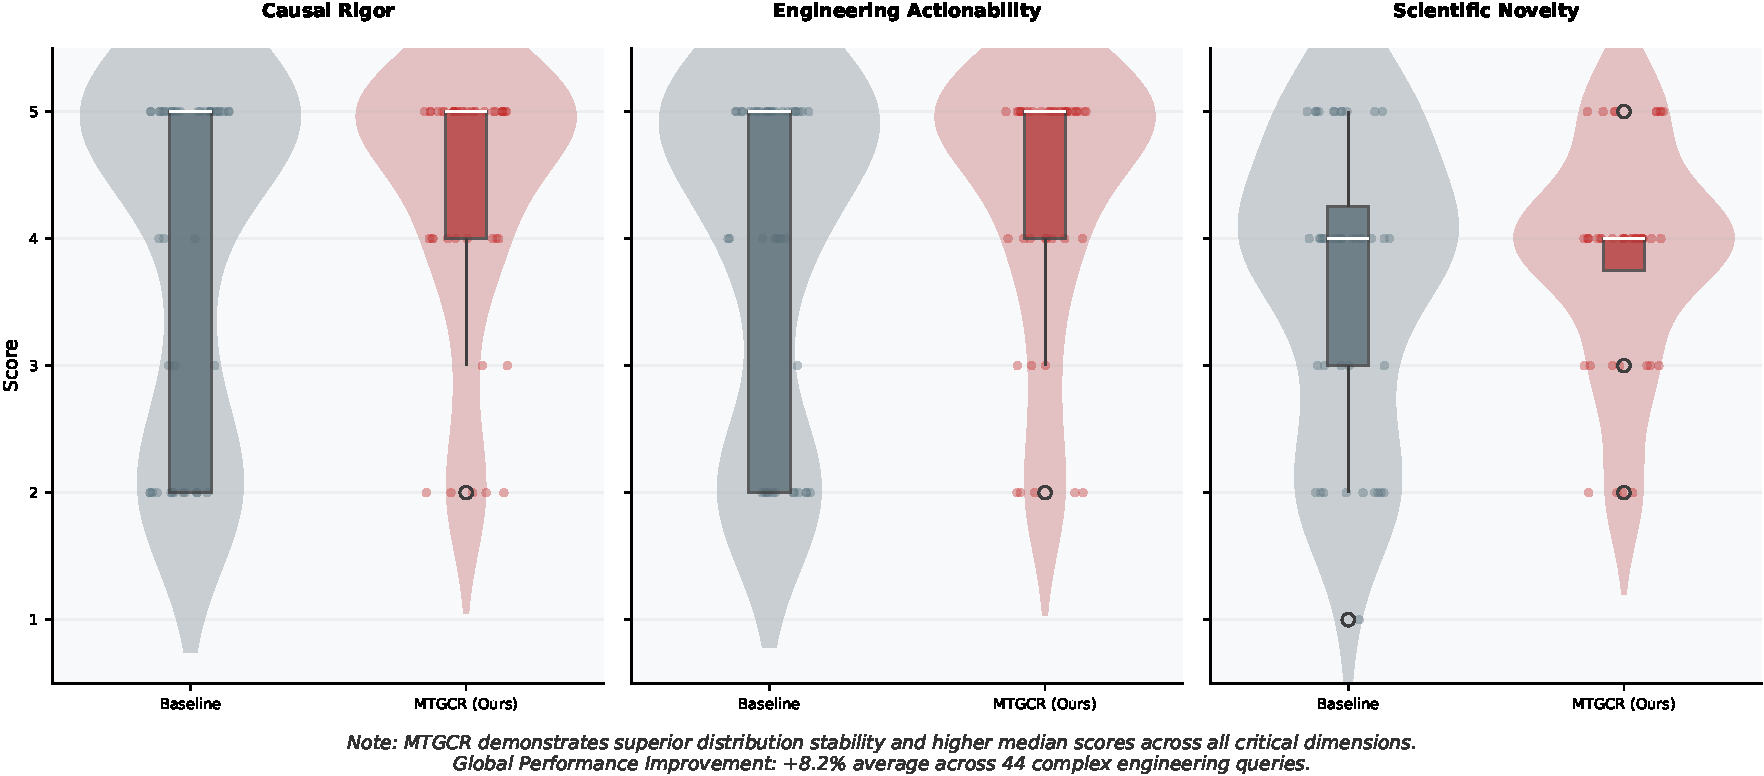
\includegraphics[width=0.95\textwidth]{ultra_premium_distribution.pdf}}
        
        \column{0.44\textwidth}
        \textbf{分布特征分析}：
        \begin{itemize}[<+->]
            \setlength{\itemsep}{0pt}
            \item \textbf{底线提升}：DRR 显著消除了 3.0 分以下的低质量回答（消灭“不知道”和“纯幻觉”）。
            \item \textbf{长尾鲁棒性}：得分分布的方差更小，中位数整体右移。
            \item \textbf{工程兜底}：由于 Critic 模块的物理常识校验，系统表现出了极高的下限稳定性。
        \end{itemize}
    \end{columns}
\end{frame}

\begin{frame}{双盲偏好评估：反向结果与深度反思}
    \small
    \begin{columns}[T,onlytextwidth] % 顶部对齐
        \column{0.44\textwidth}
        \centering
        % 加一个带阴影的边框框住图片，显得更精致
        \setlength{\fboxsep}{0pt}
        \setlength{\fboxrule}{0.5pt}
        \fcolorbox{gray!30}{white}{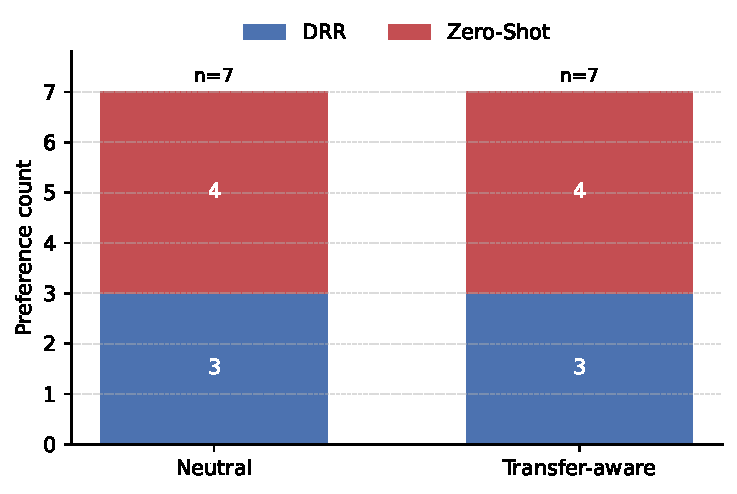
\includegraphics[width=0.75\textwidth]{blind_ab_preference.pdf}}
        
        \vspace{0.05cm}
        \begin{beamercolorbox}[wd=\textwidth, rounded=true, shadow=false, sep=0.5ex]{block body}
            \scriptsize \textbf{图表说明}：在 7 题代表性跨域子集上的双盲 A/B 测试，展示了不同评审口径下的胜率分布。
        \end{beamercolorbox}
        
        \column{0.54\textwidth}
        \textbf{评估结果}：
        \begin{itemize}
            \item \textbf{中性评审口径}：DRR vs Zero\_Shot = \alert{3 : 4}
            \item \textbf{迁移感知口径}：DRR vs Zero\_Shot = \alert{3 : 4}
        \end{itemize}
        
        \textbf{结论}：人类偏好结果与自动评分 (+10\%) 的方向\alert{完全相反}。
        
        \begin{block}{差异溯源分析}
            \footnotesize
            \begin{enumerate}[<+->]
                \setlength{\itemsep}{0pt}
                \item \textbf{冗长偏见}：LLM-as-a-Judge 偏好更长、结构更密的答案。
                \item \textbf{自我偏好}：评测器与生成器同属 Gemini 家族。
                \item \textbf{应试风险}：自动评分定义与系统显式填充字段高度重合。
            \end{enumerate}
        \end{block}
    \end{columns}
\end{frame}

% --- SECTION 5: 总结与反思 ---
\section{总结与局限性反思}

\begin{frame}{结论定调：系统设计模式}
    \textbf{研究定调}：
    本文不宣称 MTGCR 构成了具有绝对胜出优势的算法范式，而更宜将其理解为一种\textbf{“系统设计模式 (System Design Pattern)”}。
    
    \vspace{0.3cm}
    它提供了一个\alert{可运行、可审查、可回归的全栈知识平台原型}，展示了将局部机制表示与全局图谱组织结合起来，在复杂工程推理任务中的可行性证据。
\end{frame}

\begin{frame}{核心局限性与后续验证路径}
    作为严谨的学术探讨，必须承认当前工作存在以下明显局限：
    
    \vspace{0.3cm}
    \begin{itemize}[<+->]
        \item \textbf{贡献归因不可分离}：缺少 \texttt{DRR-no-tree}、\texttt{DRR-no-critic} 等逐模块消融实验，无法独立证明单一模块的边际贡献。
        \item \textbf{评测闭环与偏见}：自动评估严重受制于同家族模型的冗长偏见与自我偏好，且缺乏外部基准（如 MultiHop-RAG）的独立校验。
        \item \textbf{无统计显著性检验}：单次运行的 $\pm 0.1$ 量级差异，在未报告方差与 $p$ 值的情况下，难以排除随机扰动。
    \end{itemize}
    
    \vspace{0.3cm}
    \small \textit{这些局限性构成了后续工作（如引入 Claude 交叉验证、执行严格消融）的明确清单。}
\end{frame}

\begin{frame}[standout]
    \centering
    \Huge \textbf{答辩结束，谢谢聆听！}\\
    \vspace{0.2cm}
    \Large \textbf{敬请各位评委老师批评指正}
\end{frame}

\end{document}
